%%%%%%%%%%%%%%% Start of Title Page %%%%%%%%%%%
\begin{titlepage}
  \begin{center}
    \textit{Heaven's Light is Our Guide}
    \\[0.5cm]
    \textbf{\Large Rajshahi University of Engineering \& Technology}
    \\[0.3cm]
    \textbf{\large Department of Electronics \& Telecommunication Engineering}
    \\[0.2cm]
    \begin{figure}[!htbp]
      \centering
      
\includegraphics[scale=0.3]{src/logo_ruet}
      \label{fig:RUET logo}
    \end{figure}
    \textbf{\Large ETE 1212: Sessional Based on ETE 1211 }
    \\[0.5cm]
    \myrule[1pt][5pt]

    %%%%%%%%%%%%%%%%%%%%%%%%%%%%%%%%%%%%%%%%%%%%%%%
    %%%%%%%%%%%%%%% STUDENT'S INFO %%%%%%%%%%%%%%%%
    %%%%%%%%%%%%%%%%%%%%%%%%%%%%%%%%%%%%%%%%%%%%%%%

    \textbf{\Large  Experiment No. 01}
    \\[.25cm]
    \textbf{\large Experimental Study on Oscilloscope, Signal Generator, Project Board, Multimeter and Implementation of Simple Circuit using LED}
    \\
    \myrule[1pt][5pt]
    \begin{minipage}{0.4\textwidth}
      \vspace{0.5cm}
      \begin{flushleft}
        \emph{\textbf{\large Submitted by:}}
        \\
        Shahoriar Rahman \\
        Roll: 2104001 \\
        Session: 2021-22
      \end{flushleft}
    \end{minipage}
    ~
    \begin{minipage}{0.4\textwidth}
      \vspace{0.5cm}
      \begin{flushright}
        \emph{\textbf{\large Submitted to:}}
        \\
        Hasan Sarker
        \\
        Lecturer
        \\
        Dept. of ETE, RUET
        \\
      \end{flushright}
    \end{minipage}\\[0.7cm]
    \makeatother

    \textbf{Date of Experiment : 09/07/2023}\\
    \textbf{Date of Submission : 22/07/2023}\\[1cm]

    %************** End of Student's Info *********


    \vfill
    %%%%%%%%%%%%%%% TEACHER SECTION %%%%%%%%%%%%%%%
    \hrulefill
    \vspace{-5mm}
    \begin{multicols}{3}
      \begin{itemize} [labelindent=3em,labelsep=0.5cm,leftmargin=*,noitemsep]
        \item[] \textbf{\underline{Report}}
        \item[$\square$] Excellent
        \item[$\square$] Very Good
        \item[$\square$] Good
        \item[$\square$] Average
        \item[$\square$] Poor
      \end{itemize}
      \columnbreak
      \textbf{(Teacher's Section)}
      \\[1.5cm]
      --------------------------------
      \\
      Signature
      \columnbreak
      \begin{itemize}
        [labelindent=6em,labelsep=0.5cm,leftmargin=*,noitemsep]
        \item[] \textbf{\underline{Viva}}
        \item[$\square$] Excellent
        \item[$\square$] Very Good
        \item[$\square$] Good
        \item[$\square$] Average
        \item[$\square$] Poor
      \end{itemize}
    \end{multicols}
  \end{center}
\end{titlepage}
\newpage
%************** End of Teacher Section ********
%************** End of Title Page *************


%%%%%%%%%%%%%%% Exp. Positioning %%%%%%%%%%%%%%
\titleformat{\chapter}[display]
{\normalfont\large\bfseries}{\chaptertitlename\ \thechapter}{0pt}{\large}

\titlespacing*{\chapter}{0pt}{-15pt}{10pt}
% \addcontentsline{lof}{chapter}{\protect\numberline{ \ref{exp1}}}
% \addcontentsline{lot}{chapter}{\protect\numberline{ \ref{exp1}}}
%************** End of Exp. Positioning *******


%%%%%%%%%%%%%%%%%%%%%%%%%%%%%%%%%%%%%%%%%%%%%%%
%%%%%%%%%%%%%%% Student's Part %%%%%%%%%%%%%%%%
%%%%%%%%%%%%%%% Start of Report %%%%%%%%%%%%%%%
%%%%%%%%%%%%%%%%%%%%%%%%%%%%%%%%%%%%%%%%%%%%%%%


%**********************************************
\chapter{Observation of Ratings of Various Electrical Machines}
\label{exp1}


%**********************************************
\section{Objectives}
\begin{enumerate}
  \item To understand the functionalities of Oscilloscope, Signal Generator, Project
        Board and Multimeter.
  \item To to able to create circuit using breadboard.
  \item To understand the functionality of series and parallel circuit.
\end{enumerate}

\section{Theory}
\subsection{Oscilloscope}
\begin{figure}[H]
  \centering
  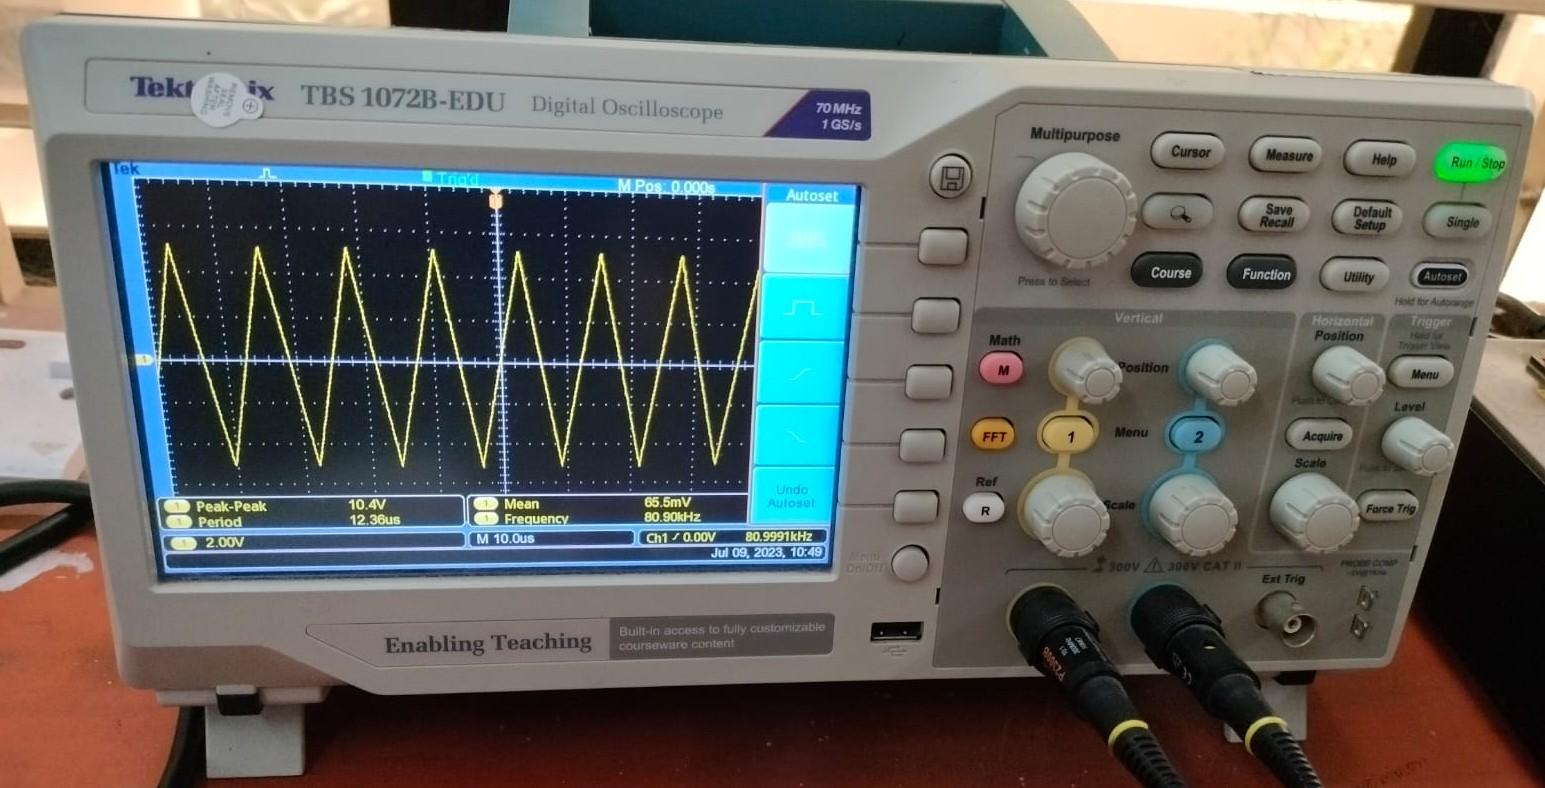
\includegraphics[scale=0.15]{src/exp01/oscilloscope.jpeg}
  \caption{An operating Oscilloscope}
\end{figure}
An oscilloscope is an electronic instrument used to measure and analyze electrical waveforms. It operates based on the principle of displaying voltage variations over time. The device takes in an electrical signal, which is typically a voltage, and converts it into a graphical representation on a screen. The vertical axis represents the voltage, while the horizontal axis represents time. By capturing and sampling the input signal, the oscilloscope generates a waveform that displays the voltage's behavior. This allows users to observe signal characteristics such as amplitude, frequency, phase, and waveform distortion. Oscilloscopes are widely used in fields like electronics, telecommunications, engineering, and scientific research for signal analysis and troubleshooting purposes.

\subsection{Signal Generator}
\begin{figure}[H]
  \centering
  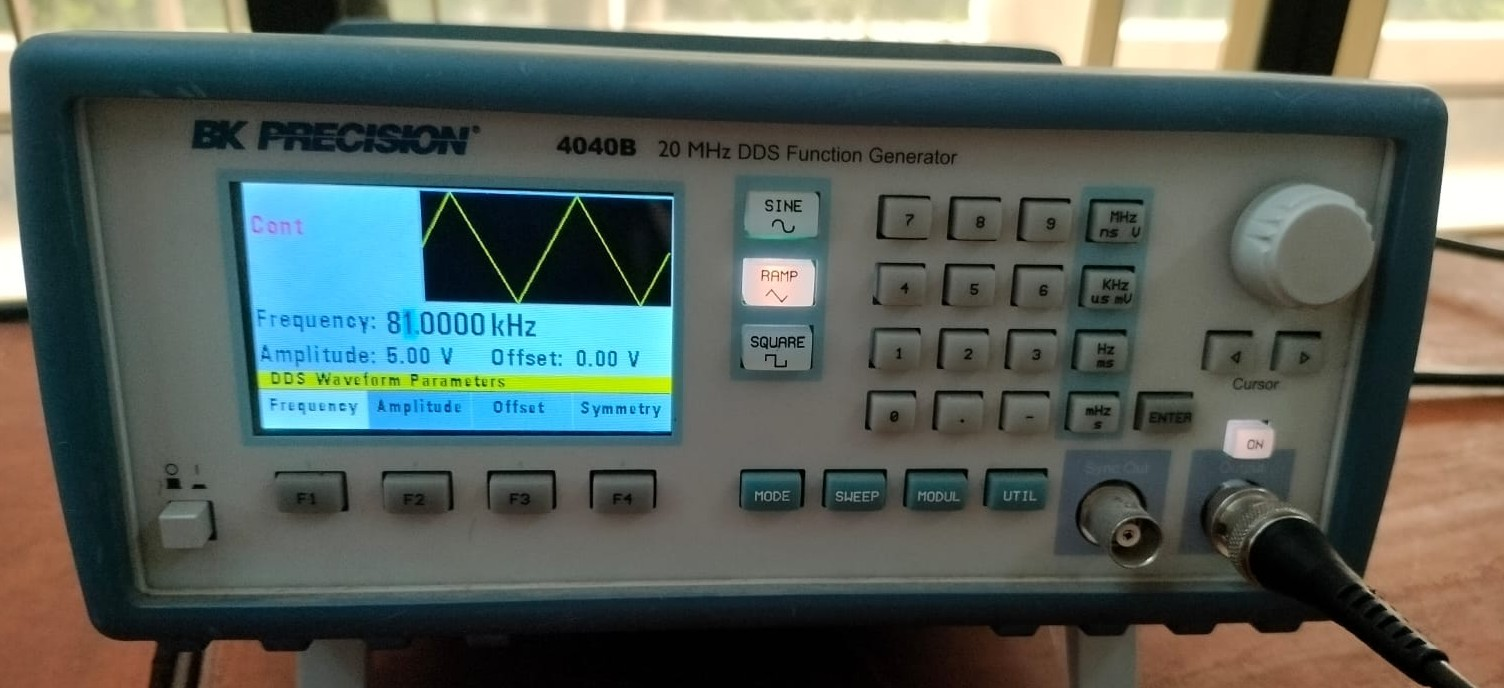
\includegraphics[scale=0.15]{src/exp01/signal_gen.jpeg}
  \caption{An operating Signal Generator}
\end{figure}
A signal generator is an electronic device used to produce various types of electrical waveforms for testing and measurement purposes. Its working principle involves generating precise and controllable signals with specific characteristics. The device typically includes oscillators that produce different types of waveforms, such as sine, square, triangle, and sawtooth waves. These waveforms are generated at specific frequencies and amplitudes based on user settings. Signal generators can also provide modulation capabilities to simulate real-world signal conditions. They are widely used in electronics, telecommunications, and research laboratories for tasks like equipment testing, circuit verification, and calibration. Their versatility and ability to produce accurate and adjustable signals make them indispensable tools in these industries.
\subsection{Project Board}
\begin{figure}[H]
  \centering
  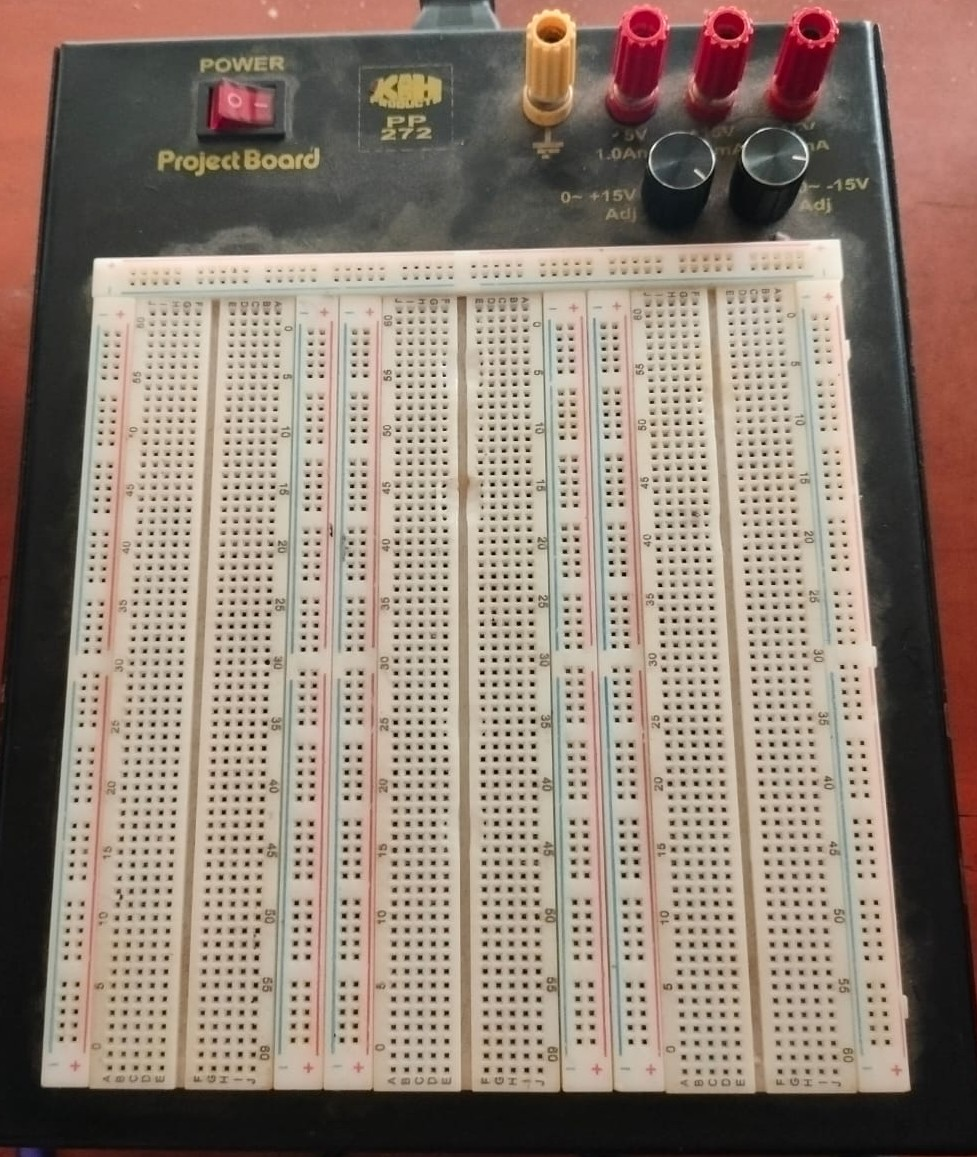
\includegraphics[scale=0.15]{src/exp01/project_board.jpeg}
  \caption{Project Board}
\end{figure}
A project board, also known as a prototyping board or breadboard, is a tool used in electronics for rapid circuit prototyping. Its working principle involves providing a platform for the temporary construction and testing of electronic circuits without the need for soldering. The project board consists of a grid of interconnected holes that can accommodate electronic components and wires. Components are inserted into the board, and wires are used to establish connections between them. The board allows for quick experimentation and modification of circuit designs, making it an essential tool for engineers and hobbyists. Its versatility and reusability make it ideal for testing and refining circuitry before committing to a permanent soldered design.
\subsection{Digital Multimeter}
\begin{figure}[H]
  \centering
  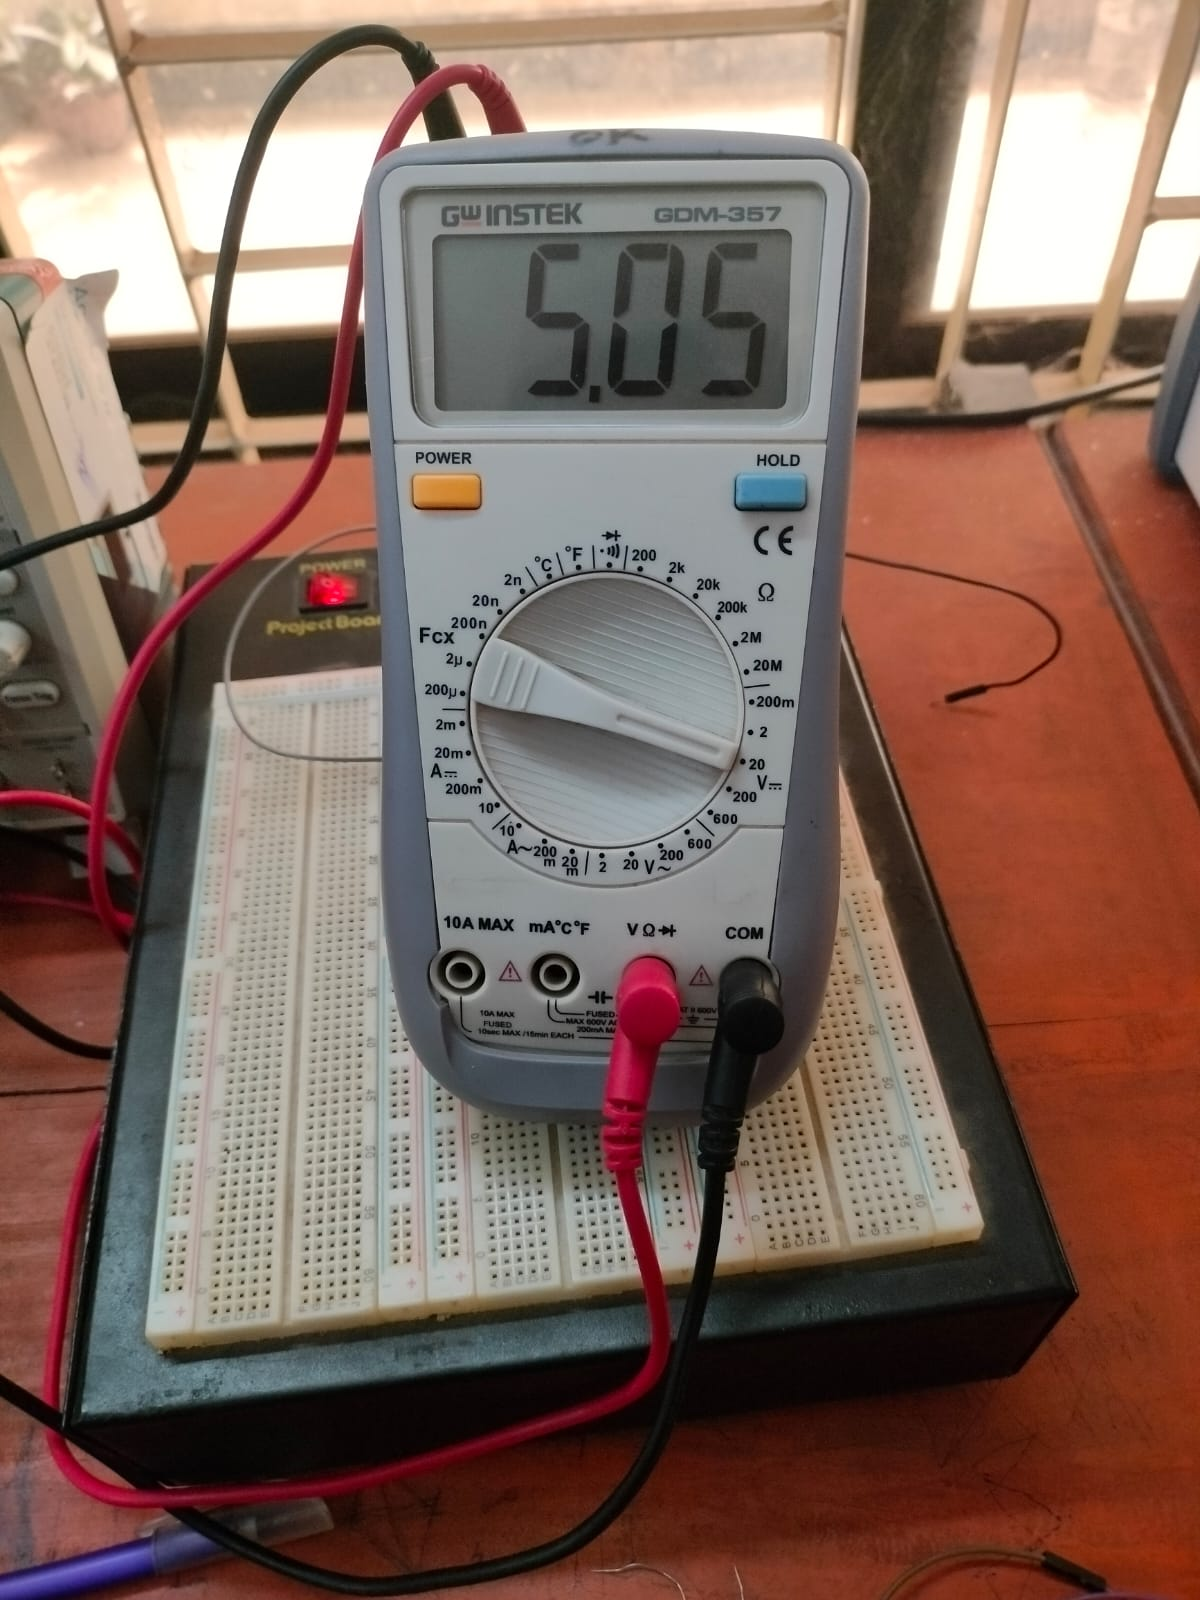
\includegraphics[scale=0.15]{src/exp01/multimeter.jpeg}
  \caption{Digital Multimeter}
\end{figure}
A multimeter is an essential electronic instrument used to measure various electrical quantities such as voltage, current, and resistance. Its working principle involves the use of internal circuits and probes to make accurate measurements. The device typically consists of a digital or analog display, selection knobs, and input jacks. When a measurement is required, the user selects the appropriate measurement mode and inserts the probes into the corresponding jacks. The multimeter then sends a known current or voltage through the circuit being tested and measures the resulting response. This allows the user to determine the electrical characteristics of the component or circuit under examination. Multimeters are widely used in electronics, electrical engineering, and troubleshooting applications for their versatility in measuring a wide range of electrical parameters.

\subsection{LED}
\begin{figure}[H]
  \centering
  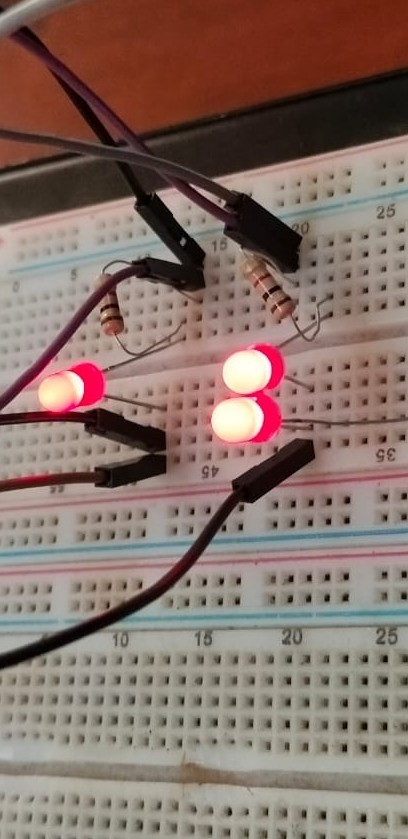
\includegraphics[scale=0.19, angle=270]{src/exp01/leds.jpeg}
  \caption{LEDs}
\end{figure}
LED (Light Emitting Diode) is a semiconductor device that emits light when an
electric current passes through it. It operates on the principle of
electroluminescence, converting electrical energy into light energy. LEDs are highly
efficient, durable, and versatile light sources. They offer significant advantages such
as energy savings, long lifespan, and resistance to shocks. LEDs are used in various
applications including lighting, displays, signage, and automotive lighting.

\subsection{Resistors}
\begin{figure}[H]
  \centering
  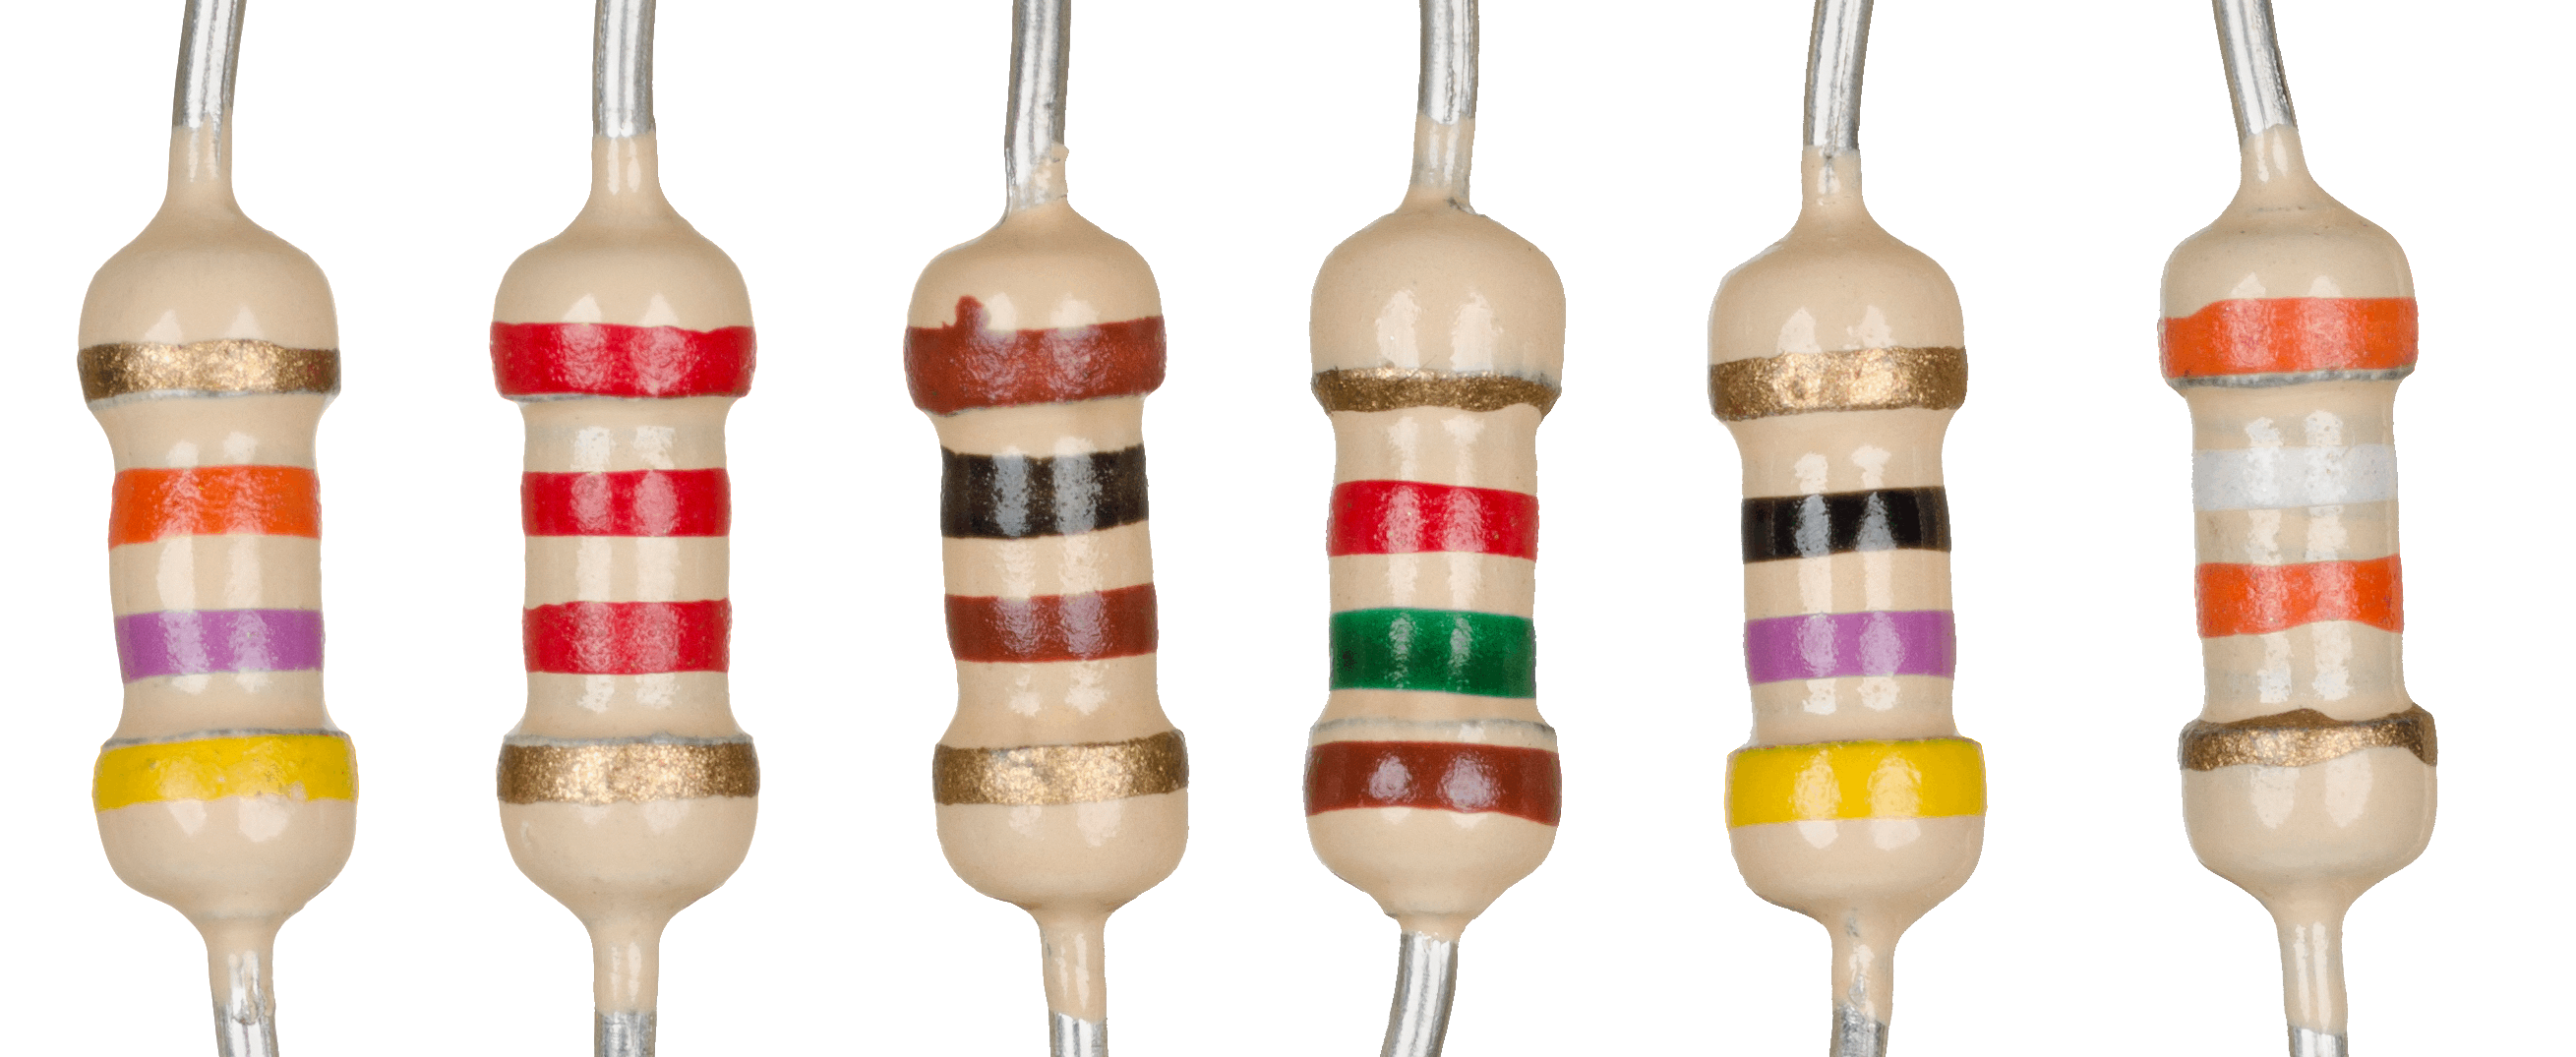
\includegraphics[scale=0.1]{src/exp01/Electronic-Axial-Lead-Resistors-Array.png}
  \caption{Resistors}
\end{figure}
A resistor is an electronic component that limits the flow of electric current in a
circuit. Its functionality revolves around its ability to resist the flow of electrons, converting electrical energy into heat. Resistor values are measured in ohms $(\Omega)$ and can be fixed or variable. By introducing resistance into a circuit, resistors control the amount of current flowing through it, protect components from excessive current, and help shape voltage levels. They are widely used in electronic circuits for current limiting, voltage division, and signal conditioning. Resistors come in various types, such as carbon composition, metal film, and wire-wound, each with its own characteristics and applications.


\section{Required Components}
\begin{enumerate}
  \item LED(s)
  \item Resistor(s)
  \item Project Board
  \item Oscilloscope
  \item Signal Generator
  \item Multimeter
  \item Jumper Cables
\end{enumerate}
\section{Circuit Diagram}
\begin{figure}[H]
  \centering
  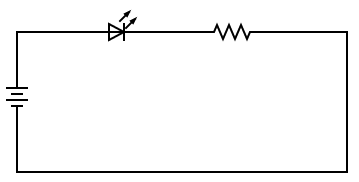
\includegraphics[scale=0.5]{src/exp01/circuit-1.png}
  \caption{Circuit Diagram with single LED and Resistor}
\end{figure}

\begin{figure}[H]
  \centering
  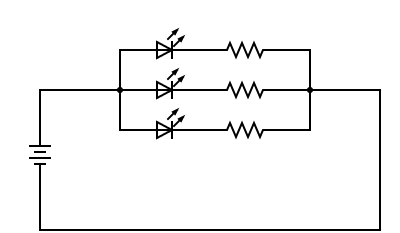
\includegraphics[scale=0.5]{src/exp01/circuit-2.png}
  \caption{Circuit Diagram with multiple LEDs and Resistors connected in parallel}
\end{figure}

\section{Experimental Data}
\begin{table}[H]
  \centering
  \renewcommand{\arraystretch}{2}
  \begin{tabular}{|c|c|c|c|c|c|}
    \hline
    \boldmath{$V_s$} & \textbf{\textbf{LED}} & \textbf{\boldmath{$V_ \text{LED}$ }} & \textbf{\boldmath{$V_R$ (V)}} & \textbf{\boldmath{$V_T$ (V)}} & \textbf{Error(\%)} \\ \hline
    5.03             & L1                    & 1.89                                 & 3.15                          & 5.04                          & 0.2                \\ \hline
  \end{tabular}
  \caption{Experimental data for only one LED and resistor connected in series with source}
\end{table}

\begin{table}[H]
  \centering
  \renewcommand{\arraystretch}{2}
  \begin{tabular}{|c|c|c|c|c|c|c|}

    \hline
    \textbf{Sl. No.} & \multicolumn{1}{c|}{\textbf{\boldmath{$V_s$ (V)}}} & \multicolumn{1}{c|}{\textbf{LED}} & \multicolumn{1}{c|}{\textbf{\boldmath{$V_ \text{LED}$ }}} & \multicolumn{1}{c|}{\textbf{\boldmath{$V_R$ (V)}}} & \multicolumn{1}{c|}{\textbf{\boldmath{$V_T$ (V)}}} & \multicolumn{1}{c|}{\textbf{Error(\%)}} \\ \hline
    1                & 5.03                                               & L1                                & 1.89                                                      & 3.13                                               & 5.02                                               & 0.2                                     \\ \hline
    2                & 5.03                                               & L2                                & 1.9                                                       & 3.11                                               & 5.01                                               & 0.4                                     \\ \hline
    3                & 5.03                                               & L3                                & 1.9                                                       & 3.1                                                & 5.00                                               & 0.5                                     \\ \hline
  \end{tabular}
  \caption{Experimental data for 3 LEDs and Resistors connected in parallel with
    source}
\end{table}
\section{Result}
Percentage of error: \\
$(E_1) = 0.2$
$(E_2) = \frac{0.2+0.4+0.5}{3} = 0.367$

\section{Discussion}
In this lab experiment, we constructed two circuits using a breadboard to
investigate the behavior of series and parallel connections, as well as to verify
Kirchhoff's Voltage Law (KVL). The first circuit consisted of an LED and a
resistor connected in series with a power source, while the second circuit involved
three series resistors and LEDs, with their series connections in parallel with the
power source.
To validate KVL, voltage measurements were taken using a digital multimeter
(DMM) across each resistor and LED in both circuits. By applying KVL, the sum
of the measured voltages across all components in a closed loop should be zero.
In the first circuit, the voltage measured across the resistor should be equal to the
voltage drop across the LED since they are in series. The sum of these two voltage
measurements should be equal to the voltage of the power source. By comparing
the calculated sum with the measured values, we can confirm whether KVL holds
true in this circuit.
In the second circuit, the voltage measurements across each resistor and LED were
taken to examine the distribution of voltage drops. The sum of these measured
voltages should also be equal to the voltage of the power source. By comparing thecalculated sum with the measured values, we can ascertain if KVL is satisfied in
this circuit as well.
During the experiment, it was observed that the measured voltage drops across the
resistors were proportional to their resistance values, confirming the expected
behavior based on Ohm's Law. The voltage drops across the LEDs were consistent
with their forward voltage specifications, indicating their proper operation.
By verifying Kirchhoff's Voltage Law, the experiment provided practical insights
into circuit analysis principles. It demonstrated the applicability of KVL and
reinforced the understanding of voltage distribution in series and parallel circuits.
Additionally, the use of a digital multimeter enabled accurate voltage
measurements, enhancing the reliability of the experimental results.

\section{Conclusion}
The lab experiment successfully explored the behavior of circuits with series and
parallel connections, while also validating Kirchhoff's Voltage Law (KVL). By
constructing two circuits on a breadboard, we examined the voltage drops across
resistors and LEDs, measuring them with a digital multimeter.
Through our observations and measurements, we confirmed that the voltage drops
across the resistors were proportional to their resistance values, in line with Ohm's
Law. The voltage drops across the LEDs were consistent with their specified
forward voltage requirements, indicating their proper functionality.
By verifying KVL, we demonstrated that the sum of voltage drops across
components in a closed loop equaled the voltage of the power source. In both
circuits, the measured voltage drops satisfied Kirchhoff's Voltage Law, providing
evidence of the law's validity in electrical circuits.
This lab experiment deepened our understanding of circuit analysis principles,
emphasizing the importance of KVL in determining voltage distribution.
Additionally, it enhanced our proficiency in using a digital multimeter for accurate
voltage measurements.
Overall, the experiment served as a practical application of theoretical concepts, allowing
us to gain hands-on experience in circuit construction, voltage measurement, and the
verification of Kirchhoff's Voltage Law.

